%%--------------------------------%
\Chapter{Approaches To Enhance Manufacturing Agility}
\label{chapter:PRICE}
%%--------------------------------%


\section{Manufacturing Environments and Systems}
\label{chapter:environments}
%\section{Traditional Manufacturing Environments}
%\label{section:environments}
Daghestani~\cite{Daghestani.1998} made an attempt to clarify the difference between manufacturing environments and manufacturing systems since a literature a review on his part showed inconsistency in the definition of these two terms. According to Daghestani~\cite{Daghestani.1998}, manufacturing environments are product-dependent. Attributes defining manufacturing environments include~\cite{Kingsman.1993,Brannon.1993,Donaldson.1995}: 1) Product characteristics. Features and functions of the product, 2) Product variety. Different types of products the company should produce, 3) Lead time. Period of time until the product enters the market, and 4) Product life cycle (PLC). Length (or number of periods) and quantity a product is in demand over its life-cycle.

The different ways the company selects to deal with these attributes in order to control the environment is referred to as a manufacturing system (equipment used, production techniques, etc). Therefore, a company can be operating under many systems at the same time.
%
%\section{Classification of Manufacturing Systems}
%Manufacturing systems can be classified according to production type, production layout and
%production volume~\cite{Leitao.2004}.
%
%\subsection{Production Type}
%The types of production, in terms of production orders, are usually divided into:
%\begin{itemize}
%\item make-to-stock~\cite{make-to-stock}, where the production is done for stock, based in forecast orders, such as in
%the high volume textile and shoe industry.
%\item assembly-to-order~\cite{make-assembly-engineer}, where final products are only assembled after receiving a customer
%order, such as the automobile industry.
%\item make-to-order~\cite{make-assembly-engineer}, where the production of the product starts after receiving a customer order,
%such as in the case of production of machine tools.
%\item engineer-to-order~\cite{make-assembly-engineer}, which is an extension of make-to-order type, where one-of-a-kind products
%are designed and manufactured according to the customer specifications, such as in
%the space electronics.
%\end{itemize}
%\subsection{Production Layout}
%Another possible classification of a manufacturing system is according to the physical plant
%layout. The factory plant layout refers to the disposition of the physical facilities in a production
%plant. The different plant layouts are fixed position, product flow layout and process layout.
%\begin{itemize}
%\item In the fixed position layout~\cite{fixed.production.layout}, the product is fixed due to its size or weight (e.g., an airplane), and the different components of the system (robots, operators, etc) go to the product to execute the operations needed to produce that product.
%\item In the product flow layout~\cite{fixed.production.layout,production.layout}, the equipment are placed through a product flow line, in order
%to minimise the transport time between machines. The transport between the workstations
%can be done manually, using automatic conveyors, robots or Automated Guided Vehicles (AGVs). This
%layout presents a reduced material transport effort, small work in progress and simple production
%planning and control system, being adequate to the mass production type. However, it presents
%small flexibility in product changes and requires high investment, due to the need to duplicate
%equipment through the flow line.
%\item In the process layout~\cite{process.layouta,process.layoutb}, the machines are grouped according to the manufacturing process,
%i.e. grouping the machines that can execute similar operations. The parts visit the several
%groups according to the specified operation sequence. This layout is adequate for the job shop
%and batch production types, presenting good flexibility and low investment in equipment with
%no need to duplicate equipment. However, it presents as disadvantages low efficiency in the
%material transportation and higher complexity in the production planning and control systems.
%\end{itemize}
%\subsection{Production Volume}
%A manufacturing system can also be classified according to the production volume. Under
%this vector it is possible to find three production types [Groover, 1987]:job shop, batch and mass production.
%\begin{itemize}
%\item The job shop production is characterised by the production of small quantities, often one-of-a-kind, of a great variety of products. Typically, the equipment used in this production type must be flexible and general purpose to support the great variety of products. As examples
%of job shop production, it is possible to mention the production of machine tools, molds and aircrafts.
%\item The batch production involves the production of lots of medium sized quantities of the same
%product, that has a regular but not so high demand. The equipment used in batch production
%is general purpose specially designed for higher production rates, for example a tool machine
%equipped with special fixtures designed to increase the machine production rate. As examples of
%items produced using batch production it is possible to find electronics equipments and furniture
%manufacturing.
%\item The mass production is related to the specialised production of one or a small number of
%products, each one with high production rates. The equipment and the factory plant used in
%mass production is completely dedicated to the production of a particular product. Examples of items produced using this type of production are screws and light bulbs.
%\end{itemize}
\section{Agile Manufacturing Environments}

The term agile manufacturing has been used by many in academia and industry as the solution to dealing with the ever-increasing turbulent and dynamic market going into the 21st century~\cite{CHO.CIE.1996}. Most literature encountered assert that agile manufacturing refers to a dynamic manufacturing setting which allows rapid reconfiguration and is highly adaptive to quick market changes through widespread use of information technology~\cite{Graves.1995,Xiaoyuan.1996}. Sharifi \& Zhang~\cite{SHARIFI.2001} viewed agility as comprising of two main factors: responding to changes in proper ways and due time, and exploiting changes and taking advantage of changes as opportunities. The authors identified high rate of new product introductions as well as quick introduction of new products as key properties of an agile manufacturing
system.

Agile manufacturing environments differ from traditional manufacturing environments in the fact that product life cycles are becoming shorter while the quest for higher qualities are becoming more consequential, and products are becoming increasingly diversified and global. Such product characteristics are becoming increasingly more prevalent and are being documented by many studies. For example, different authors report at least one of the following product characteristics~\cite{Sanderson.1990,Cordero.1991,Hisrich.1991,Millson.1992}:
\begin{itemize}
\item Decreasing concept-to-market and, thus, the introduction time between new products.
\item Decreasing length of PLCs.
\item Increasing product variety.
\item Decreasing volumes for identical products.
\end{itemize}

\section{Agile Manufacturing Systems}

Goldman \textit{et al.}~\cite{Goldman.1994} defined an agile manufacturing system as a system that is capable of operating profitably in a competitive environment of
continually and unpredictably changing customer opportunities. Tsourveloudis \& Valavanis~\cite{Tsourveloudis.2002} regarded the main capabilities of an
agile production system as the ease with which the system can change between products, and the ability to introduce new products without investments. According to Elkins \textit{et al.}~\cite{Elkins.2004}, agile manufacturing systems for engine and transmission
machining applications will permit fast cost-effective responses to unpredictable and ever-changing product demand, and support rapid product launches for previously unplanned products tailored to meet changing customer desires. Quinn \textit{et al.}~\cite{QUINN.1997} has adopted a definition of agile manufacturing that applies to light mechanical assembly of products made from components in part families: \emph{Agile manufacturing is the ability to accomplish changeover between the manufacture of different assemblies}. Rapid changeover is defined as the ability to move from the assembly of one product to the assembly of a similar product with a minimum of change in tooling and software.


\subsection{Robotic Assembly Systems}
In recent years there has been considerable interest in assembly planning and robotic systems for assembly manufacturing. Hu \textit{et al.}~\cite{Hu.2011} define assembly as the capstone process for product realization where component parts and subassemblies are integrated together to form the final products. At the more abstract Assembly Planning level, an assembly plan is a sequence of assembly tasks that start in a state where all parts are unconnected and terminates in a state representing the final assembled product. At this level each task is specified in terms of assembly parts or sub-assemblies, with no reference to production line resources or tools. At the Control Planning level each assembly task is broken down into steps, each one corresponding to an assembly robot operation. A control plan is a sequence of control tasks that start in a state where all parts are unconnected and all resources are available for assembly and terminates in a final state with the product fully assembled. Each task at this level is specified in terms of assembly parts (or sub-assemblies) and production system resources, and therefore, control plans require knowledge about system resources.

A robot, according to the Robot Institute of America, is \emph{A reprogrammable multifunctional manipulator designed to move material, parts, tools, or specialized devices through various programmed motions for the performance of a variety of tasks}. Therefore, because of their re-programmability and adaptability aspects, robots are suited to many requirements or
applications associated with industrial tasks~\cite{Kumar.2012}.



As such, many efforts study how to efficiently integrate robotic solutions in assembly systems. Below is a classification of robots used in manufacturing robotic assembly systems.

\subsubsection{Industrial Robots}
A literature review on manufacturing assembly systems mainly shows efforts describing industrial robots. The different types of industrial robots used in manufacturing assembly can be categorized as follows (based on manipulator geometry)~\cite{industrial-robots}:
\begin{itemize}
\item Cartesian robots/Gantry robots~\cite{Majors.Gantry.1997} are used for pick and place work, application of sealant, assembly operations, handling machine tools and arc welding. Cartesian robots/Gantry robots consist of an arm with three prismatic joints and whose axes are coincident with a Cartesian coordinator.
\item Cylindrical robots~\cite{Geering.Cylindrical.1986} are used for assembly operations, handling at machine tools, spot welding, and handling at diecasting machines. Cylindrical robots consist of axes that form a cylindrical coordinate system.
\item SCARA robots~\cite{Yao.SCARA.1999} are used for pick and place work, application of sealant, assembly operations and handling machine tools. SCARA robots consist of two parallel rotary joints to provide compliance in a plane.
\item Articulated robots~\cite{Puiu.Articulated.2009} are mainly used for assembly operations, diecasting, fettling machines, gas welding, arc welding and spray painting. Articulated robots consist of an arm that has at least three rotary joints.
\item Parallel robots~\cite{Khalil.Parallel.2011} are mainly used for pick and place work and assembly operations. Parallel robots consist of arms that have concurrent prismatic or rotary joints.
\end{itemize}


\subsubsection{Mobile Robots}
Besides industrial robots, mobile robots have been introduced in modern manufacturing systems~\cite{Lazinica.Mobile.2005a,Lazinica.Mobile.2005b,Angerer.Mobile.2012,Delrobaei.Mobile.2009}. Such robots should be autonomous, adaptable, and function smoothly in order to cope with unstructured and highly complex manufacturing systems. Mobile robots are used for: 1) Transport: Mobile robots are used as carriers for assembling products. This function is performed with the use of autonomous mobile robots with exchangeable pallets. 2) Assembly: Mobile robots with manipulator and part storage for different assembly parts. 3) Supply: Delivering of assembly parts to assembly stations. This function is usually performed by autonomous mobile robots that adapt to  transport assembly parts in quantities. 4) Load: Positioning of assembly pallet on transport robot. 5) Unload: Removing the assembly pallet of the finished product from the transport robot.

\section{Use Cases}
\label{sec:uses}
Robots have long held a pre-eminent place in high-volume, high-capital industries such as auto manufacturing, but recent advances in robots' brawn and brains have seen their use expand into many new industries. This section will look at recent applications for small and large part assembly, advances in 3D vision, and trajectory optimization. The citations in this section come from published whitepapers and use cases from robotics manufacturers \href{http://new.abb.com/products/robotics}{ABB}, \href{http://www.fanucamerica.com/default.aspx}{Fanuc}, \href{http://www.kuka-robotics.com/usa/en/}{Kuka}, and \href{http://www.motoman.com/index.php}{Yaskawa}.

A common yet challenging task for industrial robots is the assembly of systems and subsystems from smaller components, often selected from bins or kits. Automotive applications are still a staple of industrial robotics, but apart from heavy-lifting assembly operations such as vehicle axles \cite{ABB4} or engine cylinder heads \cite{ABB3}, smaller systems such as brake assemblies \cite{Yaskawa1} or lighting fixtures \cite{Yaskawa2} are also being assembled by robotic workers. Similarly, small electromechanical systems can now be assembled with high-speed, high-precision systems, including televisions \cite{ABB1}, meters \cite{Fanuc1}, or key fobs \cite{Fanuc4}.

In addition to traditional realms of employment, assembly robots are carving out new niches in emerging fields demanding precision and reliability while still seeking to scale production economically. For example, fuel cell assembly can be accelerated with specialized robots \cite{Kuka1}, leading to cost and reliability improvements. Robots have even made their way into sewing carbon fiber cloth for use in aircraft \cite{Kuka2}.

Finally, new technologies are transforming the way even traditional robot tasks are performed. For instance, performance of already installed an running platforms can be improved with online trajectory characterization and learning \cite{Fanuc2}, or by re-optimizing in simulation without shutting down production for manual teaching \cite{Fanuc3}. Similarly, advances in 3D perception are enabling robots to deal with more challenging pick-and-place environments by performing object recognition on the pieces to be assembled \cite{ABB2}.

All of these advances are beginning to see field deployment, and are ready for wider adoption. In the next sections, we will look instead at capabilities that are under active development, but are likely to drive the next wave of advanced robotic applications.

\section{Hardware Abstraction}
\label{sec:abstraction}
A principal characteristic of a mature technology industry is the ability to design a system at a relatively high level, then implement the abstract design using standard (sometimes parameterized) tools. However, too many current robotic installations are built with ad-hoc, non-transferable code. In order to be able to design systems at a higher level, engineers need a unified way of describing robots, tasks, and objects in such a way that the hardware implementation details need not be hard-coded into the design details. The following sections highlight various methods for designing general systems to run on specific platforms.


\subsection{Robot Ontologies}
A robot ontology defines the framework within which a robotic system can characterize its world. Having a shared and comprehensive vocabulary with which to describe itself, its tasks, and its environment is a prerequisite for robots that seek to collaborate with one another, and for engineers who wish to create extensible behaviors at a more abstract level. Thus, it is important for such frameworks achieve broad adoption in order to be useful to the robots and their programmers.

A number of attempts at defining these robot world frameworks have been made over the years, varying in scope and application. A major effort currently underway is described in
\cite{Schlenoff2012a}, % ieee organizational logistics
an IEEE-sponsored effort which lays out goals of describing a core robot world language and several specific use cases.
Another ongoing project is the RoboEarth framework, described in
\cite{Tenorth2013a},
which outlines the creation of a ``Wikipedia for robotics'', encompassing robot and object descriptions as well as skill level descriptions intended to be shared on robot-to-robot via the Internet.

% Robot and Object Libraries
Often, ontology definitions may specialize into defining robot taxonomies, as seen in
\cite{Schlenoff2005a} % rescue robot classes
and
\cite{Schlenoff2005},
where explicitly delineating the classes into which an agent can fall is a major focus that enables determining utility for various tasks.
Other variations highlight the ability to execute a specific skill or behavior, whether for manipulator robots, as in
% Skill Libraries
\cite{Huckaby2013},
or for additive manufacturing, such as
\cite{Liu2010}. % 3d printing layers
Of course, some knowledge representations seek to model both of these aspects, as well as defining classes for environmental objects, as in
% Both
\cite{Tenorth2013}. % KnowRob knowledge base
\subsection{Cloud Robotics}
Another enabling technology for escaping the bonds of single-purpose robot installations is the emerging field of cloud robotics, introduced by James Kuffner from Google and CMU \cite{Guizzo2011}. In these systems, robots gain increased capabilities from being connected either to the Internet, or to a large intranet. A primary purpose of this connectivity is access to the knowledge databases defined in the previous section, with particular examples including the RoboEarth/KnowRob projects in
% Access to mentioned libraries
\cite{Tenorth2013} % KnowRob knowledge base
and
\cite{Tenorth2013a}.

% Distributed processing
In addition, connection to a network allows for the deployment of robots with lower onboard computational capability, as intensive calculations can be directed to a dedicated server. This can drive lower development and deployment costs, as computationally heavy tasks such as object recognition \cite{Kehoe2013} or motion planning in a cluttered environment \cite{Hunziker2013} can be performed on well-equipped machines, perhaps sporting multiple GPUs or other computation tools. This also centralizes design and maintenance work, allowing high-level software changes to be decoupled from the specifics of each robot installation.

Finally, traditional roles for cloud computing can be leveraged in a a robotics context. For instance, cloud-based data backup \cite{Hookings2013} or operational data collection and reporting \cite{Hookings2013b} are common IT paradigms currently being applied to industrial robots by several manufacturers. These techniques enable easier management of fleets of robots for even smaller businesses.

\subsection{ROS-Industrial}
Finally, no discussion of hardware-agnostic robot development would be complete without highlighting the ongoing ROS-Industrial project \cite{Edwards2012}. ROS-I is a project that strives to adapt the Robot Operating System (ROS) popular for academic research to the industrial community. This allows for faster integration of research breakthroughs, as well as access to a broad spectrum of computer vision, motion planning, and robot control tools. For example, MoveIt!, the ROS-based motion planning framework, currently supports nearly 50 robot platforms
\cite{MoveItUserCommunity2014}.





\section{Process Adaptability}
\label{sec:adaptability}
An important concern for small-medium enterprises considering a robotic installation is their traditionally smaller batch size and greater process variability. In addition to the programming developments mentioned in Section \ref{sec:abstraction}, several research trends over the past decade have investigated methods for increasing this process-level flexibility. When these concerns are well managed, powerful new applications can be realized for challenging domains \cite{Spencer1996}.

\subsection{Managing Variability}
Industrial robots tend to be known for their extreme precision, but this precision is wasted if the object to be operated on has far more variability than the operating robot. Fortunately, this variation can be modelled and handled by closing the loop on manufacturing processes.

Much of the research on managing variation focuses on modelling and propagating position errors at a given step, ex.
\cite{Mantripragada1999},
\cite{Zhou2003},
\cite{Liu2010a}.
The assembly process is usually modelled using a state-space formulation, with the process error being described by a (probabilistic) state transition model. Those familiar with Kalman filtering will recognise the roles of process and measurement noise models and their incorporation into the true state estimate. The final error is often represented by a differential motion vector.

However, simply modelling error propagation is insufficient to solve the problem. Knowing the expected error bounds enables closing the loop at a further step in the process. In
\cite{Balakirsky2013},
sensor feedback is combined with a system ontology to identify and correct errors. In general, machine vision provides loop closure for many robotic systems, and advances in 3D sensing hardware and algorithms are driving powerful 3D-reconstruction based adaptive systems.

\subsection{Mass Customization}
One of the major trends in agile manufacturing is the flexibility to handle small batches of a product, allowing for production of a greater variety of items, as well as better responsiveness to new product lines. In the extreme case this becomes known as mass customization, where each item is tailor-made for a customer's order
\cite{Piller2004},
\cite{Fogliatto2012}.

The ROSETTA Project
\cite{Patel2012}
is one project seeking to improve robot flexibility in this sector. Major focuses of the project include boosting ease of programming (Section \ref{sec:abstraction}) and simplifying robot integration into human systems (Section \ref{sec:collaboration}).

\pagebreak
\section{Human Interaction}
\label{sec:humans}
Most SME robotic installations cannot dedicate a massive warehouse to their mechanized workers, nor dominate their current workspace with extensive safety cages and barriers. Additionally, robots are not yet dexterous enough for certain tasks, so human involvement may be required at various stages in the pipeline. Thus, robots need to play nicely with their biological coworkers
\cite{Dong2011}.

\subsection{Workspace Collaboration and Human Safety}
\label{sec:collaboration}
At the forefront of considerations when integrating robots into a workflow is the issue of worker safety. Traditionally, industrial robots have been massive, rigid machines able to achieve high precision in the presence of disturbance forces, with little regard to whether the disturbance came from a process variation or from a coworker who had strayed too close. Two major focuses of work in this area are in risk analysis and mechanical compliance .

At one end of the safety spectrum is the concept of provably safe, in which a robot cannot cause harm to even an intentional human actor
\cite{Mitsch2013} % provably safe
Other sources, such as
\cite{Kulic2006}. % Danger index
prefer to compute a measure of the risk in the current system, termed a danger index. Similarly,
\cite{Lacevic2013} % danger field
incorporates a danger field, which defines operating regions where the robot must be afforded the most respect.

Manufacturers are also aware of the growing desire for closer human-robot interaction. A newer generation of robotic arms incorporates human safety into the mechanical design
\cite{UniversalRobots}, % VW
enabling better worker collaboration
\cite{Knight2013} % MIT TR BMW
without requiring proofs of algorithm safety.
Finally, work is underway to certify different classes of worker safety in the presence of industrial robots
\cite{Matthias2011}, \cite{Fryman2012}.

Once issues of safety have been handled, discussion can proceed on how best to integrate human and mechanical workers.
\cite{Kruger2009} %
and
\cite{Tan2009}
give case studies examining how to efficiently integrate the two sides of the manufacturing system to boost productivity while maintaining safety.

\subsection{Learning from Demonstration}
One of the more exciting developments in the field of human-robot collaboration is the possibility of teaching the robot with no programming from the operator. Such learning research has been underway for some time (see
\cite{Argall2009}
for a review), but the technology is finally maturing to the point of entering commercial products. Perhaps the most famous instance of this is the Baxter robot
\cite{Fitzgerald2013},
although other manufacturers are beginning to incorporate similar learning systems, such as the Kinetiq learning system being developed by Robotiq and Yaskawa
\cite{Kinetiq2013},
\cite{Kinetiq2013b-url}.
% List # of robots
% Strengths
% Weaknesses 


\begin{figure}[!htb]
\begin{center}
        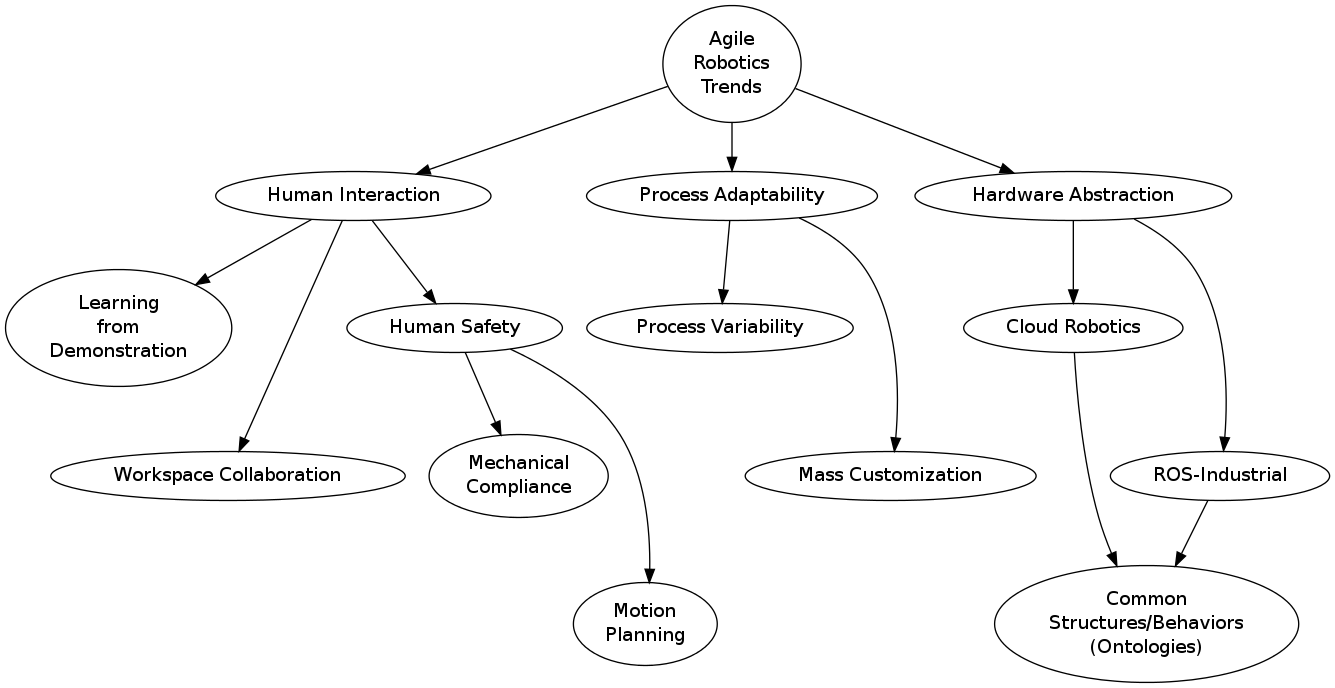
\includegraphics[width=1.0\linewidth]{Figures/topics1.png}
\caption{Topic Hierarchy with Associated References.}
\label{fig:refGraph}
\end{center}
\end{figure}
\begin{figure}[!htb]
\begin{center}
        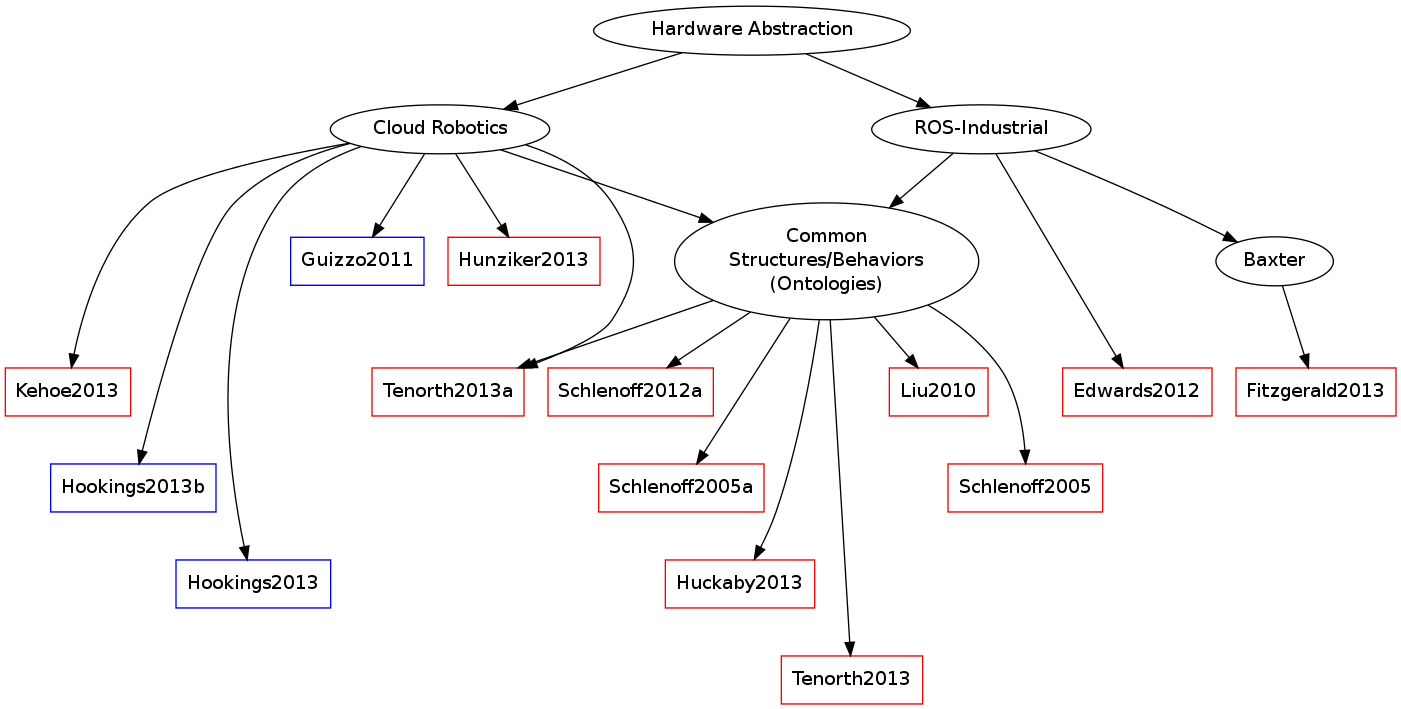
\includegraphics[width=1.0\linewidth]{Figures/topics2.png}
\caption{Topic Hierarchy with Associated References. (continued)}
\label{fig:refGraphA}
\end{center}
\end{figure}
\begin{figure}[!htb]
\begin{center}
        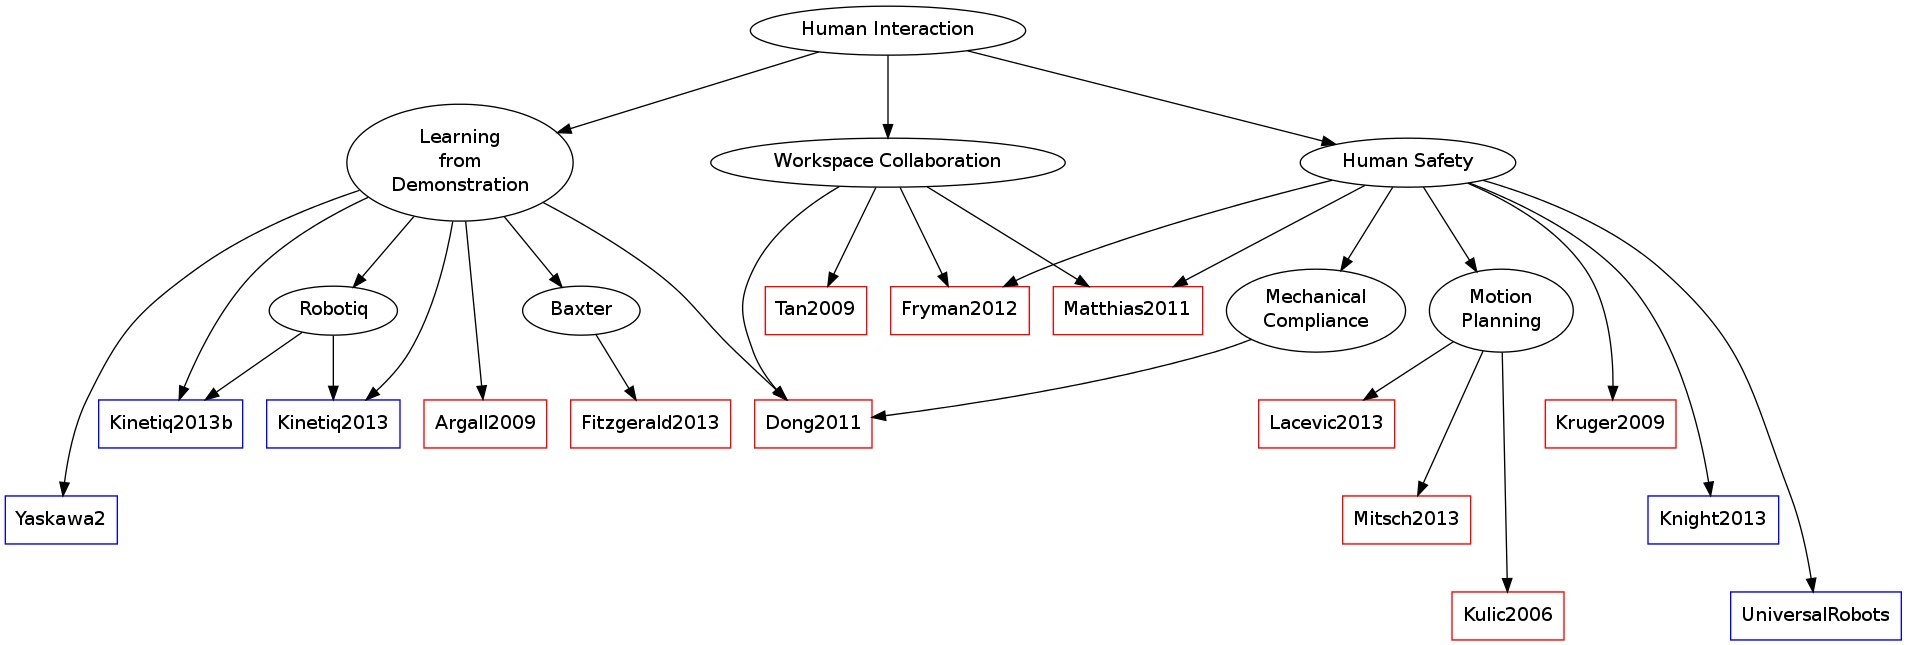
\includegraphics[width=1.0\linewidth]{Figures/topics3.png}
\caption{Topic Hierarchy with Associated References. (continued)}
\label{fig:refGraphB}
\end{center}
\end{figure}
\begin{figure}[!htb]
\begin{center}
        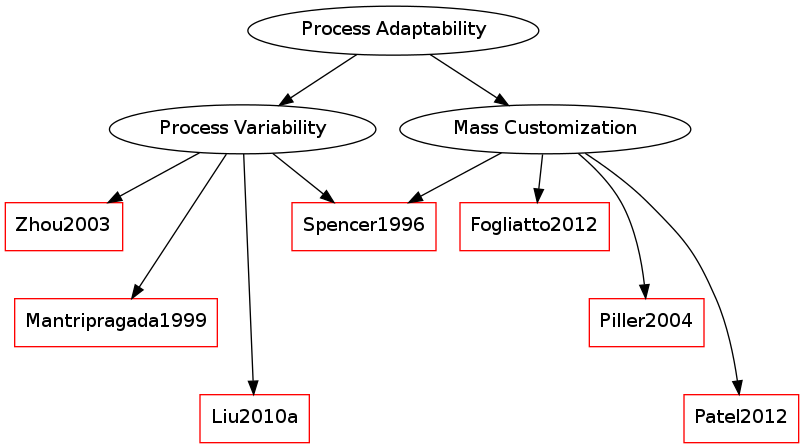
\includegraphics[width=0.6\linewidth]{Figures/topics4.png}
\caption{Topic Hierarchy with Associated References. (continued)}
\label{fig:refGraphC}
\end{center}
\end{figure}
\pagebreak